% Options for packages loaded elsewhere
% Options for packages loaded elsewhere
\PassOptionsToPackage{unicode}{hyperref}
\PassOptionsToPackage{hyphens}{url}
%
\documentclass[
  ignorenonframetext,
  twocolumn]{beamer}
\newif\ifbibliography
\usepackage{pgfpages}
\setbeamertemplate{caption}[numbered]
\setbeamertemplate{caption label separator}{: }
\setbeamercolor{caption name}{fg=normal text.fg}
\beamertemplatenavigationsymbolsempty
% remove section numbering
\setbeamertemplate{part page}{
  \centering
  \begin{beamercolorbox}[sep=16pt,center]{part title}
    \usebeamerfont{part title}\insertpart\par
  \end{beamercolorbox}
}
\setbeamertemplate{section page}{
  \centering
  \begin{beamercolorbox}[sep=12pt,center]{section title}
    \usebeamerfont{section title}\insertsection\par
  \end{beamercolorbox}
}
\setbeamertemplate{subsection page}{
  \centering
  \begin{beamercolorbox}[sep=8pt,center]{subsection title}
    \usebeamerfont{subsection title}\insertsubsection\par
  \end{beamercolorbox}
}
% Prevent slide breaks in the middle of a paragraph
\widowpenalties 1 10000
\raggedbottom
\AtBeginPart{
  \frame{\partpage}
}
\AtBeginSection{
  \ifbibliography
  \else
    \frame{\sectionpage}
  \fi
}
\AtBeginSubsection{
  \frame{\subsectionpage}
}
\usepackage{iftex}
\ifPDFTeX
  \usepackage[T1]{fontenc}
  \usepackage[utf8]{inputenc}
  \usepackage{textcomp} % provide euro and other symbols
\else % if luatex or xetex
  \usepackage{unicode-math} % this also loads fontspec
  \defaultfontfeatures{Scale=MatchLowercase}
  \defaultfontfeatures[\rmfamily]{Ligatures=TeX,Scale=1}
\fi
\usepackage{lmodern}

\usetheme[]{tud}
\ifPDFTeX\else
  % xetex/luatex font selection
\fi
% Use upquote if available, for straight quotes in verbatim environments
\IfFileExists{upquote.sty}{\usepackage{upquote}}{}
\IfFileExists{microtype.sty}{% use microtype if available
  \usepackage[]{microtype}
  \UseMicrotypeSet[protrusion]{basicmath} % disable protrusion for tt fonts
}{}
\makeatletter
\@ifundefined{KOMAClassName}{% if non-KOMA class
  \IfFileExists{parskip.sty}{%
    \usepackage{parskip}
  }{% else
    \setlength{\parindent}{0pt}
    \setlength{\parskip}{6pt plus 2pt minus 1pt}}
}{% if KOMA class
  \KOMAoptions{parskip=half}}
\makeatother


\usepackage{longtable,booktabs,array}
\usepackage{calc} % for calculating minipage widths
\usepackage{caption}
% Make caption package work with longtable
\makeatletter
\def\fnum@table{\tablename~\thetable}
\makeatother
\usepackage{graphicx}
\makeatletter
\newsavebox\pandoc@box
\newcommand*\pandocbounded[1]{% scales image to fit in text height/width
  \sbox\pandoc@box{#1}%
  \Gscale@div\@tempa{\textheight}{\dimexpr\ht\pandoc@box+\dp\pandoc@box\relax}%
  \Gscale@div\@tempb{\linewidth}{\wd\pandoc@box}%
  \ifdim\@tempb\p@<\@tempa\p@\let\@tempa\@tempb\fi% select the smaller of both
  \ifdim\@tempa\p@<\p@\scalebox{\@tempa}{\usebox\pandoc@box}%
  \else\usebox{\pandoc@box}%
  \fi%
}
% Set default figure placement to htbp
\def\fps@figure{htbp}
\makeatother


% definitions for citeproc citations
\NewDocumentCommand\citeproctext{}{}
\NewDocumentCommand\citeproc{mm}{%
  \begingroup\def\citeproctext{#2}\cite{#1}\endgroup}
\makeatletter
 % allow citations to break across lines
 \let\@cite@ofmt\@firstofone
 % avoid brackets around text for \cite:
 \def\@biblabel#1{}
 \def\@cite#1#2{{#1\if@tempswa , #2\fi}}
\makeatother
\newlength{\cslhangindent}
\setlength{\cslhangindent}{1.5em}
\newlength{\csllabelwidth}
\setlength{\csllabelwidth}{3em}
\newenvironment{CSLReferences}[2] % #1 hanging-indent, #2 entry-spacing
 {\begin{list}{}{%
  \setlength{\itemindent}{0pt}
  \setlength{\leftmargin}{0pt}
  \setlength{\parsep}{0pt}
  % turn on hanging indent if param 1 is 1
  \ifodd #1
   \setlength{\leftmargin}{\cslhangindent}
   \setlength{\itemindent}{-1\cslhangindent}
  \fi
  % set entry spacing
  \setlength{\itemsep}{#2\baselineskip}}}
 {\end{list}}
\usepackage{calc}
\newcommand{\CSLBlock}[1]{\hfill\break\parbox[t]{\linewidth}{\strut\ignorespaces#1\strut}}
\newcommand{\CSLLeftMargin}[1]{\parbox[t]{\csllabelwidth}{\strut#1\strut}}
\newcommand{\CSLRightInline}[1]{\parbox[t]{\linewidth - \csllabelwidth}{\strut#1\strut}}
\newcommand{\CSLIndent}[1]{\hspace{\cslhangindent}#1}



\setlength{\emergencystretch}{3em} % prevent overfull lines

\providecommand{\tightlist}{%
  \setlength{\itemsep}{0pt}\setlength{\parskip}{0pt}}



 


% Use fontspec to load Noto Emoji
\usepackage{fontspec}

% Define Noto Emoji font for emojis
\newfontfamily\emojiFont{Twitter Color Emoji}
\newfontfamily\fallbackFont{DejaVu Sans}

% Automatically switch to emoji font for unicode emoji characters
\newcommand{\emoji}[1]{{\emojiFont #1}}
% Command for fallback font
\newcommand{\fallback}[1]{{\fallbackFont #1}}

\usepackage[ruled,vlined]{algorithm2e}
\makeatletter
\@ifpackageloaded{tcolorbox}{}{\usepackage[skins,breakable]{tcolorbox}}
\@ifpackageloaded{fontawesome5}{}{\usepackage{fontawesome5}}
\definecolor{quarto-callout-color}{HTML}{909090}
\definecolor{quarto-callout-note-color}{HTML}{0758E5}
\definecolor{quarto-callout-important-color}{HTML}{CC1914}
\definecolor{quarto-callout-warning-color}{HTML}{EB9113}
\definecolor{quarto-callout-tip-color}{HTML}{00A047}
\definecolor{quarto-callout-caution-color}{HTML}{FC5300}
\definecolor{quarto-callout-color-frame}{HTML}{acacac}
\definecolor{quarto-callout-note-color-frame}{HTML}{4582ec}
\definecolor{quarto-callout-important-color-frame}{HTML}{d9534f}
\definecolor{quarto-callout-warning-color-frame}{HTML}{f0ad4e}
\definecolor{quarto-callout-tip-color-frame}{HTML}{02b875}
\definecolor{quarto-callout-caution-color-frame}{HTML}{fd7e14}
\makeatother
\makeatletter
\@ifpackageloaded{caption}{}{\usepackage{caption}}
\AtBeginDocument{%
\ifdefined\contentsname
  \renewcommand*\contentsname{Table of contents}
\else
  \newcommand\contentsname{Table of contents}
\fi
\ifdefined\listfigurename
  \renewcommand*\listfigurename{List of Figures}
\else
  \newcommand\listfigurename{List of Figures}
\fi
\ifdefined\listtablename
  \renewcommand*\listtablename{List of Tables}
\else
  \newcommand\listtablename{List of Tables}
\fi
\ifdefined\figurename
  \renewcommand*\figurename{Figure}
\else
  \newcommand\figurename{Figure}
\fi
\ifdefined\tablename
  \renewcommand*\tablename{Table}
\else
  \newcommand\tablename{Table}
\fi
}
\@ifpackageloaded{float}{}{\usepackage{float}}
\floatstyle{ruled}
\@ifundefined{c@chapter}{\newfloat{codelisting}{h}{lop}}{\newfloat{codelisting}{h}{lop}[chapter]}
\floatname{codelisting}{Listing}
\newcommand*\listoflistings{\listof{codelisting}{List of Listings}}
\makeatother
\makeatletter
\makeatother
\makeatletter
\@ifpackageloaded{caption}{}{\usepackage{caption}}
\@ifpackageloaded{subcaption}{}{\usepackage{subcaption}}
\makeatother

\usepackage{bookmark}
\IfFileExists{xurl.sty}{\usepackage{xurl}}{} % add URL line breaks if available
\urlstyle{same}
\hypersetup{
  pdftitle={Your Title},
  pdfauthor={Your name},
  hidelinks,
  pdfcreator={LaTeX via pandoc}}


\title{Your Title}
\author{Your name}
\date{2025-01-01}

\begin{document}
\frame{\titlepage}


\section{title}\label{title}

\begin{frame}{Start with Why?}
\phantomsection\label{start-with-why}
Test1

\pause 

Text2
\end{frame}

\begin{frame}{Start with Why?}
\phantomsection\label{start-with-why-1}
\begin{center}
\includegraphics[width=0.8\textwidth]{./img/prosem-einleitung.png}
\end{center}
\end{frame}

\begin{frame}{Markmap Mindmap}
\phantomsection\label{markmap-mindmap}
\note{Frameworks in other domains - HaluEval systematically test and
measure hallucination bias in various models - Repoformer ICML 24
selective RAG for Code Completion

Other fields to draw inspot from - Customer Service Chatbots utilize
RAG}

	\begin{center}
	\vspace*{-2cm}% adjust vertical spacing before
	\hspace*{-0.9cm}% shift left by 0.5cm
	\raisebox{5.3cm}{% shift up by 0.3cm
	\resizebox{1.3\linewidth}{!}{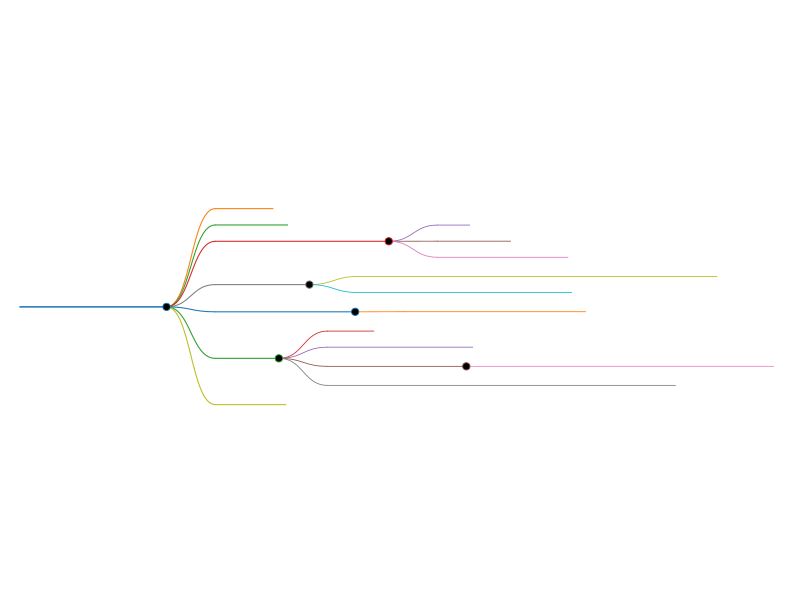
\includegraphics{img/mindmap.pdf}}
	\vspace*{-1cm}% adjust vertical spacing before
	}%
	\end{center}
	
\end{frame}

\begin{frame}{Slide 3}
\phantomsection\label{slide-3}
And svg:
\includegraphics[width=\linewidth,height=0.4\textheight,keepaspectratio]{slides_files/mediabag/img/subarrayid_page1.pdf}

Test3
\end{frame}

\begin{frame}{Small Font}
\phantomsection\label{small-font}
\begingroup

\tiny 

Tiny text..

\endgroup
\end{frame}

\begin{frame}{Callout}
\phantomsection\label{callout}
\begin{quote}
{[}!question{]} Warning

TEST-IDX123
\end{quote}

\begin{tcolorbox}[enhanced jigsaw, colback=white, rightrule=.15mm, leftrule=.75mm, bottomrule=.15mm, toptitle=1mm, toprule=.15mm, breakable, bottomtitle=1mm, opacitybacktitle=0.6, arc=.35mm, colframe=quarto-callout-note-color-frame, coltitle=black, title=\textcolor{quarto-callout-note-color}{\faInfo}\hspace{0.5em}{Tip with Title}, colbacktitle=quarto-callout-note-color!10!white, left=2mm, titlerule=0mm, opacityback=0]

My private note\ldots.

\end{tcolorbox}
\end{frame}

\section{Neue Section}\label{neue-section}

\begin{frame}{HMMM}
\phantomsection\label{hmmm}
\end{frame}

\begin{frame}{Twocols}
\phantomsection\label{twocols}
This is how to specify several cols on a slide:

\begin{columns}[T]
\begin{column}{0.4\linewidth}
contents\ldots{}
\end{column}

\begin{column}{0.6\linewidth}
contents\ldots{}
\end{column}
\end{columns}
\end{frame}

\begin{frame}{Extra Symbols}
\phantomsection\label{extra-symbols}
\begin{itemize}
\tightlist
\item
  ✓ 🧠, 📙
\item
  Other alphabets: ソ, Я
\end{itemize}

``my quote'' \citeproc{ref-PXJVWCSQ}{{[}1{]}}
\end{frame}

\begin{frame}{Mermaid}
\phantomsection\label{mermaid}
\includegraphics[width=3.56in,height=5.07in]{slides_files/figure-beamer/mermaid-figure-1.png}
\end{frame}

\begin{frame}{LaTeX algorithm2e Package}
\phantomsection\label{latex-algorithm2e-package}
\begin{algorithm}[H]
\SetAlgoLined
\KwData{Logic Network}
\KwResult{SubarrayAssignment: \[ NodeId \to \mathcal{P}(S) \]}
 initialization\;
 \While{condition}{
  instructions\;
 }
 \caption{Example algorithm}
\end{algorithm}
\end{frame}

\section{End}\label{end}

\begin{frame}{End}
\end{frame}

\begin{frame}[allowframebreaks]{References}
\phantomsection\label{references}
\footnotesize

\phantomsection\label{refs}
\begin{CSLReferences}{0}{0}
\bibitem[\citeproctext]{ref-PXJVWCSQ}
\CSLLeftMargin{{[}1{]} }%
\CSLRightInline{F. Gao, G. Tziantzioulis, and D. Wentzlaff,
{``ComputeDRAM: In-memory compute using off-the-shelf DRAMs,''} in
\emph{Proceedings of the 52nd annual IEEE/ACM international symposium on
microarchitecture}, in MICRO '52. New York, NY, USA: Association for
Computing Machinery, Oct. 2019, pp. 100--113. doi:
\href{https://doi.org/10.1145/3352460.3358260}{10.1145/3352460.3358260}.
Available: \url{https://dl.acm.org/doi/10.1145/3352460.3358260}.
{[}Accessed: Jul. 16, 2025{]}}

\end{CSLReferences}
\end{frame}




\end{document}
